\chapter{Hardware} \label{chap:hardware}
\begin{chapquote}{Donald Knuth, \textit{The Art of Computer Programming, Vol. I}}
People who are more than casually interested in computers should have at least some idea of what the underlying hardware is like. Otherwise the programs they write will be pretty weird.
\end{chapquote}

%\timos{Overall this section is ok, I think it could be improved by providing more background first, i.e., describing the target board a little bit first (instead of later in the testbed description) and introducing components, i.e., what is \ac{axi}, \ac{axi}-Lite etc. Fig 3.1 is already really detailed and at that point not understandable, maybe have an overview figure first that shows less components but clearly says "data path" and "control path". (Note that I only read the HW section, so if this is provided / planned to be in a section before, this might be fine.)
%I also missed some mapping of described things to code, this could be a simple comment to Fig 3.1 that the names in the blocks correspond to file names where this functionality is implemented. But think of this thesis as documentation that someone who wants to improve on what you did will read.}

As we introduced in \Cref{sec:background-pspin}, P\acs{spin} is a RISC-V-based packet processing cluster implementing the \ac{spin} in-network-computing paradigm.  However, P\acs{spin} itself does not consist of a fully functional SmartNIC due to the lack of capability to receive and send packets; it also lacks an interface to read from and write to the system memory.  The following three classes of hardware components need to be implemented to achieve full functionality of a \ac{spin} \ac{nic}: 

\begin{itemize}
    \item the \emph{data path}: the P\acs{spin} cluster should be able to receive packet data from the network and send a reply back into it;
    %\timos{Why is sending data optional? I guess it means not every receive is followed by a send, but it reads weird, since the sentence starts with describing capabilities.}
    \item the \emph{control path}: the P\acs{spin} cluster and other components should be configured from the host over various control registers and program memory (code and data); and finally,
    \item the \emph{host-side \ac{dma}}: the P\acs{spin} cluster should be able to read from and write to the main memory on the host system to establish the full \ac{spin} programming model.
\end{itemize}

An overview of all the hardware components is shown in \Cref{fig:hw-overview}.  We now walk through the design and implementation of these modules in more detail.

\begin{table}[ht]
    \centering
    \begin{tabular}{ll}
    \toprule
    Module Name & Description \\ \midrule
    \texttt{pspin\_host\_dma} & Host ac{dma} adapter \\
    \texttt{pspin\_ingress\_datapath} & Collective ingress data path wrapper \\
    \texttt{pspin\_her\_gen} & \ac{her} generator \\
    \texttt{pspin\_ingress\_dma} & Ingress \ac{dma} engine \\
    \texttt{pspin\_pkt\_alloc} & Packet buffer allocator \\
    \texttt{pspin\_pkt\_match} & Packet matching engine \\
    \texttt{pspin\_ctrl\_regs} & Control registers adapter \\
    \texttt{pspin\_egress\_dma} & Egress \ac{dma} engine \\
    \bottomrule
    \end{tabular}
    \caption{Description of the modules shown in in \Cref{fig:hw-overview}.} \label{tab:mod-name-desc}
\end{table}

\begin{figure}
    \centering
    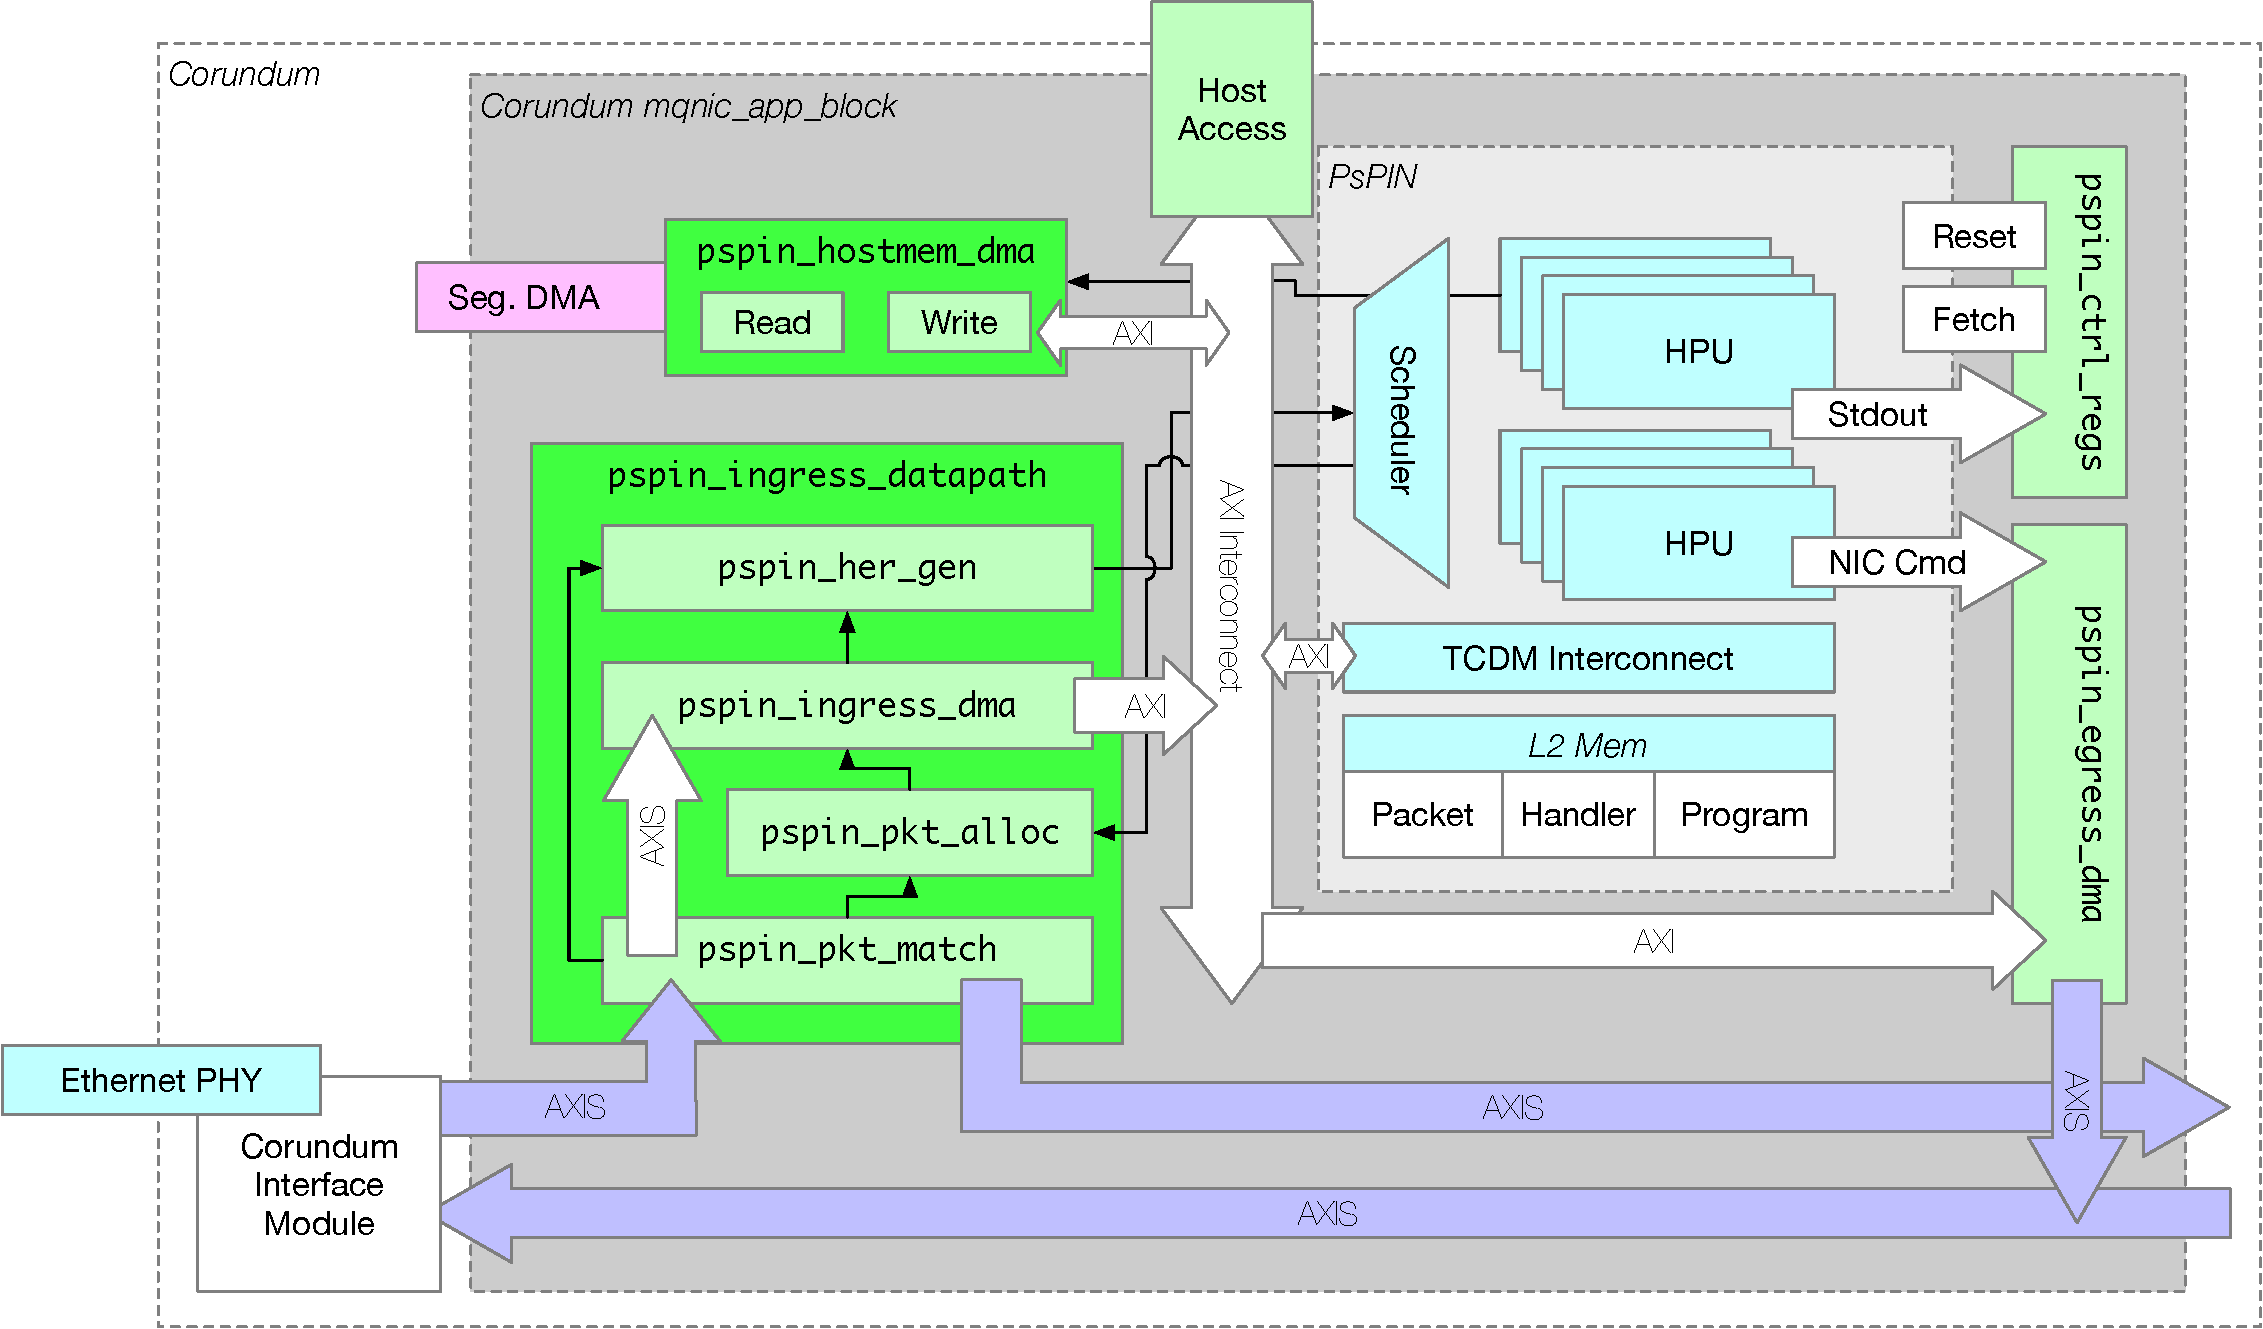
\includegraphics[width=\linewidth]{figures/hw-overview.pdf}
    \caption{Overview of the FP\acs{spin} hardware.  A description of the hardware function blocks is shown in \Cref{tab:mod-name-desc}.  Blocks marked in green are the modules implemented as part of this project to bridge the P\acs{spin} cluster to Corundum.}
    \label{fig:hw-overview}
\end{figure}

%\pengcheng{distinguish control path/data path from control flow/data flow of P\acs{spin} discussed in \Cref{sec:background-pspin}.  Brief diagram to highlight which part of the flow we are talking about}

\section{Control Path} \label{sec:hw-control}

The control path handles configuration of the P\acs{spin} cluster as well as the various data path components \emph{before} the actual execution of handler code on the cluster.  There are three important control-path tasks to perform from the host, all of which are implemented over Corundum's slow-path 32-bit \ac{axi}-Lite (\Cref{sec:fpga-basics}) interface with an address bus of 16 bits:

\begin{itemize}
    \item to toggle various control registers to the P\acs{spin} cluster and data path components;
    \item to read back standard output produced by P\acs{spin} (i.e., \texttt{printf}); and
    \item to load program code and data onto memory in the P\acs{spin} cluster.
\end{itemize}

\paragraph{Control registers} The control registers are configured through the \texttt{pspin\_\-ctrl\_\-regs} module.  The module exposes an \ac{axi}-Lite slave towards the \ac{axi}-Lite interconnect and converts this into simple \texttt{valid}-guarded interfaces (\Cref{sec:fpga-basics}) for P\acs{spin} and various data path components to consume.  Some signal groups have requirements on \emph{consistency of update}, that is, the signals in the same group should always be consistent and no partial updates should be visible to the components being controlled.  Checks for this requirement happens in the kernel driver as we will introduce in \Cref{sec:app-kmod}.  An overview of the exposed control signals from \texttt{pspin\_\-ctrl\_\-regs} is shown in \Cref{tab:ctrl-signals}.

\begin{table}[ht]
    \centering
    \begin{tabular}{lcl}
    \toprule
    Name & Direction & Description \\ \midrule
    \texttt{cl\_fetch\_en} & O & Fetch-enable control to P\acs{spin} \\
    \texttt{aux\_rst} & O & Auxiliary reset for P\acs{spin} and data path \\
    \texttt{cl\_busy} & I & Cluster busy status from P\acs{spin} \\
    \texttt{mpq\_full} & I & \ac{mpq} full status bitmap \\
    \texttt{match\_*} & O & Matching engine configuration \\
    \texttt{her\_gen\_*} & O & \ac{her} generator configuration \\
    \texttt{stdout\_*} & O & Standard output readback \\
    \bottomrule
    \end{tabular}
    \caption{Overview of the control wires exported by \texttt{pspin\_ctrl\_regs}.  The meaning of these control wires will be introduced in the coming sections.}
    \label{tab:ctrl-signals}
\end{table}

The control registers module is designed to allow reconfiguration during normal operation of the system.  Therefore, components that take configuration data from the module are expected to have a explicit \emph{valid} signal, if they expect consistency between multiple registers.  The software that controls these register would then de-assert valid, change the registers, and then reassert valid, such that the downstream module can have a consistent configuration.

\begin{figure}
    \centering
    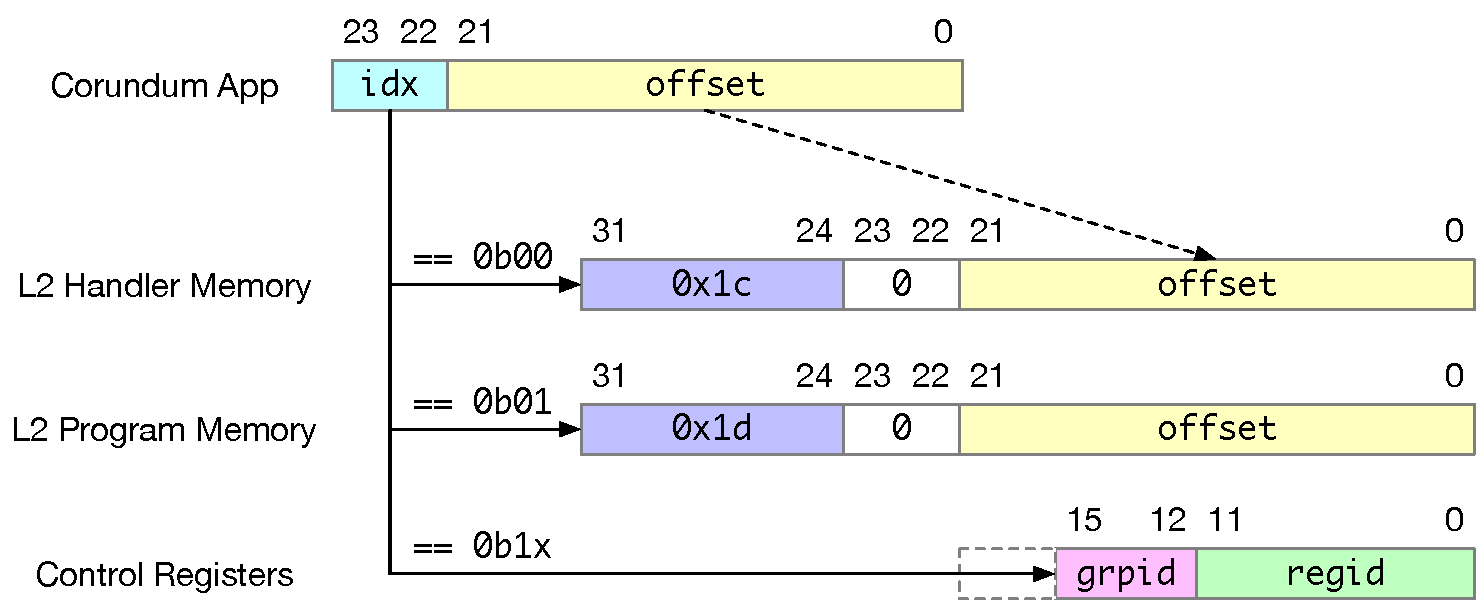
\includegraphics[width=.8\textwidth]{thesis/figures/corundum-pspin-addr.pdf}
    \caption{Address translation from the Corundum application control space.  Access to the P\acs{spin} host access space always have the top bit as 0; we use the second top bit to select the correct memory area in P\acs{spin}.  Access to the configuration registers have the top bit set to 1; the 22-bit offset is decoded as the 16-bit control register address and the top 6 bits ignored.} \label{fig:hw-addr-map}
\end{figure}

We group registers by the subsystem they control (e.g. the matching engine or the \ac{her} generator) and assign a block of address in the control register address space.  We then refine these groups into subgroups that each of them control a specific field of configuration; some of the subgroups contain multiple identical register instances (e.g. for multiple rulesets in the matching engine).  As shown in \Cref{fig:hw-addr-map}, the 16-bit control register address uses the top 4 bits ("grpid") to address the register groups and the lower 12 bits ("regid") to address the subgroup and register instances.  We do not explicitly define a subgroup field in the address due to different subgroup sizes across different groups.

To maintain consistency about the naming, word size, and addressing about various registers, we define registers in a declarative approach with an external generator (\texttt{regs-compiler.py}).  The hierarchical organisation of registers is demonstrated by the metadata describing all the registers, shown in \Cref{lst:reg-meta}.  The generator allocates addresses in the register address space w.r.t.\ the group-subgroup abstraction described in the paragraph above.

\begin{listing}[tp]
\begin{minted}{py}
groups = [
    RegGroup('cl', [
        RegSubGroup('ctrl',     False, 2),
        RegSubGroup('fifo',     True,  1),
    ]),
    RegGroup('me', [
        RegSubGroup('valid',    False, 1, 1),
        RegSubGroup('mode',     False, 4, 1),
        RegSubGroup('idx',      False, 16, 32),
        RegSubGroup('mask',     False, 16, 32),
        RegSubGroup('start',    False, 16, 32),
        RegSubGroup('end',      False, 16, 32),
    ]),
    RegGroup('her_meta', [
        RegSubGroup('handler_mem_addr',   False, 4),
        RegSubGroup('handler_mem_size',   False, 4),
        RegSubGroup('host_mem_addr',      False, 4, 64),
        RegSubGroup('host_mem_size',      False, 4),
        RegSubGroup('hh_addr',            False, 4),
        RegSubGroup('hh_size',            False, 4),
        # ... more subgroups ...
    ]),
    # ... more groups ...
]
\end{minted}
\caption{A simplified excerpt of the metadata definition of control registers in FP\acs{spin}.  \texttt{RegGroup} defines the name and children (subgroups) of the register group; \texttt{RegSubGroup} defines the name, immutability (from the CPU), number of registers, and optionally the signal width in hardware of the subgroup.  These are later consumed by Verilog and C templates to generate the register definition and use sites.} \label{lst:reg-meta}
\end{listing}

Verilog modules that interact with the control register system are written in a template language, namely Jinja~\cite{noauthor_jinja_nodate}, that abstracts the exact register definitions away.  A generator written in Python processes all Verilog templates w.r.t.\ the register metadata and emits the final source file ready for synthesis.  Such an approach eliminates the tedious and error-prone maintenance of repetitive register definitions and proved to be crucial as the number of control wires grows.  The generator also derives part of the kernel driver that later exposes these control registers as described later in \Cref{sec:app-kmod}.

\paragraph{Standard output access} To facilitate debugging of handler code on the P\acs{spin} cluster, we implement a readback mechanism for the characters printed by the RISC-V cores.  The core executes \texttt{putchar} to write characters into the \texttt{apb\_stdout} module.  Different cores write to separate addresses exported by the module, allowing the module to demultiplex the incoming characters.  The module enqueues the characters toegether with the source core ID in a \ac{fifo}.  The \ac{fifo} is then read out from \texttt{pspin\_ctrl\_regs}.  To avoid introducing module ports on all levels of \ac{rtl} hierarchy, we utilise the \emph{hierarchical reference scope}~\cite{noauthor_verilog_nodate} feature of Verilog to connect the output ports from \texttt{apb\_stdout} directly.  Finally, the host can read back the enqueued characters by reading out the \texttt{stdout\_*} registers through the register interface, demultiplex, and store the output as logs for future inspection.

\paragraph{Code and data download} The code and data of the packet handler program on P\acs{spin} need to be loaded into the \emph{program memory} in P\acs{spin} before we can start scheduling packets to execute on the HPUs.  The program memory is accessible through the \emph{host slave} port on the P\acs{spin} cluster.  This port also allows write to the other memory area, the \emph{handler memory}, to allow writing either static or dynamic configuration data by the host.  Together, this allows loading compiled P\acs{spin} program images onto the cluster memory.

We implement such access by connecting the upstream \ac{axi}-Lite port from Corundum, through a \ac{axi}-Lite interconnect and a \ac{axi}-Lite to \ac{axi}4 adpater, to the host slave port.  Note that the P\acs{spin} host access address space on the host slave port is 32-bits.  However, we only have a 24-bit address space from the application block control port from Corundum.  Therefore, we perform a \emph{compression} in the address space by mapping the two memory areas closer together into the application control port address space; we demonstrate this in \Cref{fig:hw-addr-map}.  The FP\acs{spin} kernel module (\Cref{sec:app-kmod}) will encode the P\acs{spin} memory accesses according to this mapping.

\section{Data Path}

P\acs{spin}, being a packet processor, needs to have access to the receive and transmit paths in the \ac{nic} to function properly.  We introduce in this section the design and implementation of the ingress and egress data path engines that gives P\acs{spin} access to the packet data path.

\paragraph{Attach points of the data path} Corundum provides access to raw Ethernet frames over the \ac{axi} Stream interface.  Three attachment points are available to the application block for reading ingress Ethernet frames out, as well as injecting egress frames:

\begin{itemize}
    \item \emph{Direct}: the \ac{axi} Stream interface directly after the Ethernet MACs and before most Corundum modules.  The interfaces are synchronous to the MAC clock (322.265625 MHz for 100 Gbps Ethernet).  This offers the lowest possible latency from the application block.
    \item \emph{Sync}: the \ac{axi} Stream interface after the \ac{cdc} \ac{fifo} for each port.  These interfaces are synchronous to the Corundum core clock (250 MHz).  They offer comparatively low latency.
    \item \emph{Interface}: the \ac{axi} Stream interface after the main packet aggregation \ac{fifo} per interface.  These interfaces are per interface (instead of per port; for example a 100 Gbps interface could be split into 4 25 Gbps ports, as described in \Cref{sec:fpga-basics}) and are the simplest to process.  They are synchronous to the Corundum core clock (250 MHz).
\end{itemize}

The \ac{fpga} board we use, as described in \Cref{sec:fpga-basics} and later in detail in \Cref{sec:eval-setup}, has two 100 Gbps interfaces; each interface can be further split up into 4 25 Gbps ports.  For simplicity of implementation, we attach the P\acs{spin} data path at the \emph{interface} attach point, such that we don't have to multiplex traffic from different ports by ourselves.

\subsection{Ingress} \label{sec:ingress-datapath}

After a packet has arrived at the \emph{interface} attach point, multiple tasks need to be done for an ingress packet before it lands in P\acs{spin} memory and is ready for processing.  We implement four separate functional blocks as follows; together they form the ingress data path module (\texttt{pspin\_\-ingress\_\-datapath}):

\begin{itemize}
    \item \texttt{pspin\_\-pkt\_\-match}: match if the packet is to be processed by the SmartNIC cluster or to be forwarded to the normal Corundum data path;
    \item \texttt{pspin\_\-pkt\_\-alloc}: allocate buffer for the incoming packet in the L2 packet buffer, free the buffer once it finishes processing;
    \item \texttt{pspin\_\-ingress\_\-dma}: \ac{dma} write the packet data into the L2 packet buffer
    \item \texttt{pspin\_\-her\_\-gen}: generate the \ac{her} to the P\acs{spin} cluster
\end{itemize}

We explain in detail the design of these modules.  Note that common design considerations presented in \Cref{sec:hw-design-considerations} apply to these modules.

\paragraph{Packet matching engine} \texttt{pspin\_\-pkt\_\-match} exposes one \ac{axi}-Stream slave (\texttt{s\_\-axis\_\-nic\_\-*}) towards the upstream packet data that comes from the application block interface in Corundum.  It further exposes two \ac{axi}-Stream master ports towards the downstream packet processing logic.  One of them (\texttt{m\_\-axis\_\-pspin\_\-*}) forwards the matched packet data to the rest of the data path components for further processing.  In addition, the module also exposes metadata for the matched packet over a ready-valid interface (\texttt{packet\_\-meta\_\-}) providing the downstream components with the following information:

\begin{itemize}
    \item \emph{Message ID} from the \ac{slmp} packet header (see \Cref{sec:slmp} for details of the \ac{slmp} protocol), for the \ac{her} generator
    \item \emph{\ac{eom} bit} as specified by the matching ruleset, for the \ac{her} generator
    \item \emph{Ruleset ID} of the matching ruleset, for the \ac{her} generator to select the correct \ac{ectx}
    \item \emph{Length} of the packet, for the packet buffer allocator
\end{itemize}

Since we need to count the length of the packet, the packet metadata can only be generated after that the packet has been trasferred on the \ac{axi}-Stream interface.  A later stage in the data path (the ingress \ac{dma} engine) will reverse this dependency by buffering the packet data.

We adopt a simple approach to define the matching rules similar to the IPTables U32 match~\cite{cohen_iptables_nodate}.  The matching engine provides a configurable number of \emph{rulesets}.  We expose ruleset configuration to the host as control registers.  Each ruleset is defined by a configurable number of \emph{matching rules} for the \emph{matching units}, which, each one on its own, matches against a 32-bit word of the packet and produces a boolean output.  Given index $I$, 32-bit mask $M$, 32-bit start value $S$, and 32-bit end value $E$, the matching unit output is defined as:

\[
\text{Output} := S \le (\text{Packet}[4I:4I+3] \mathbin{\&} M) \le E
\]

Each ruleset defines a \emph{mode} in which the output from the matching units are combined into the match output of the ruleset.  We currently implement two modes: \texttt{MATCH\_\-AND}, which combines the match unit outputs with a logical AND; and \texttt{MATCH\_\-OR}, for a logical OR.  The module is designed such that it is easy to add another combination mode, if such a use case rises (for example an \emph{exactly-one} combination mode).  If any of the installed rulesets matched on the packet, the module marks the packet as matched for further processing in the data path.  The module then sets the \emph{ruleset ID} metadata of the packet accordingly for \ac{ectx} selection as described later when we introduce the \ac{her} generator.

A few examples of common matching rules are as follows:
\begin{itemize}
    \item \texttt{RULE\_IP}: match EtherType at byte 12-13 = \texttt{0x0800} $\rightarrow$ matcher \#3, mask \texttt{0xffff0000}, range \texttt{0x08000000-0x08000000}
    \item \texttt{RULE\_IP\_PROTO}: match IP protocol at byte 23 = 17 (\acs{udp}) $\rightarrow$ matcher \#5, mask \texttt{0xff}, range \texttt{0x11-0x11}
    \item \texttt{RULE\_UDP\_DPORT}: match UDP destination port at byte 36-37 = 9330 (\acs{slmp}) $\rightarrow$ matcher \#5, mask \texttt{0xffff0000}, range \texttt{0x24720000-0x24720000}
    \item \texttt{RULE\_FALSE}: match nothing $\ge$ 1 and $<$ 0 (logic false) $\rightarrow$ matcher \#0, mask \texttt{0x0}, range \texttt{0x1-0x0}
\end{itemize}
%\timos{Nice explanation, maybe add an example?}

The other \ac{axi}-Stream master interface (\texttt{m\_\-axis\_\-nic\_\-*}) performs a \emph{pass-through} of packets that did not match with any installed rulesets back into the regular Corundum packet data path.  This allows the \ac{nic} with P\acs{spin} attached to it to still function as a normal \ac{nic} when P\acs{spin} is not configured.  It also enables host processing of traffic that is not of interest to P\acs{spin}, for example in handling the \ac{arp} as described in \Cref{sec:l3-protocol-handling}, or when implementing an application-level control plane in the \ac{mpi} Datatypes application as described in \Cref{sec:mpi-datatypes-demo}.

\paragraph{Packet buffer allocator} The packet buffer allocator takes the metadata from the matching engine and allocates a buffer for the packet in the L2 packet buffer of P\acs{spin}.  It runs the allocation algorithm based on the packet length, adds the resulting address of the allocated buffer to the packet metadata, and forwards the metadata to the \ac{dma} engine to actually write the packet into the memory.  It takes in the \emph{feedback} from P\acs{spin}, which denotes that a packet has been processed and its buffer can be freed, to free the buffer correctly.  It further outputs one statistics counter of how many packets have been dropped due to the buffer being full.

The Verilator model originally developed in the P\acs{spin} project uses a software-based ring buffer in the simulation testbench to allocate space for incoming packets in the packet buffer.  The free algorithm needs to keep a queue of out-of-order frees and is thus difficult to implement in hardware.  However, most packets on the Internet and in data center environments follow a \emph{bimodal} distribution in size: 40\% of packets are below 64 bytes and another 40\% are 1500 bytes (the \ac{mtu} of an Ethernet/IP network)~\cite{john_analysis_2007,benson_understanding_2009}.  We thus take a simpler \emph{fixed-size} allocation approach: we partition the packet buffer into two halves; in one half we make fixed 128-byte slots, and in the other half we make 1536-byte slots.  We store these free slots in two separate \ac{fifo}s.  We then handle allocation and free simply by popping from and pushing to the respective \ac{fifo}s.  This way, we greatly simplify the hardware implementation of the allocator while not sacrificing too much buffer utilisation on internal fragmentation.

%\pengcheng{(how) do we claim against fragmentation?  should we state that we can just increase the size of the packet buffer?}
%\timos{Do we care? We can simply say we also partition the packet buffer in two regions, one for small and one for large packets, then there is no fragmentation problem. If you mean internal fragmentation (an allocated packet might not always be fully used) ignore it.}

\paragraph{Ingress \ac{dma}} The ingress \ac{dma} module takes the allocated address and length in the packet metadata and performs a \ac{dma} transaction to write the packet data to the P\acs{spin} \ac{nic} inbound memory port.  Upon finish of the \ac{dma} request, the module forwards the packet metadata on to the \ac{her} generator in the data path, such that the packet can get scheduled on the P\acs{spin} cluster.  We use the \texttt{axi\_\-dma\_\-wr} module from the Corundum \ac{axi} IP library to perform the actual \ac{dma} operation.

One complication to be handled in this module is that the matching engine could only generate the packet metadata \emph{after} transferring the packet data on the \ac{axi}-Stream bus.  This is due to a dependency introduced by needing to count the length of the message.  While this is handled by introducing a shallow \texttt{axis\_\-fifo} to reverse this dependency for the \ac{dma} module, it would introduce a per-packet latency of the number of cycles it takes to transmit the packet on the \ac{axi}-Stream bus.  In addition, the module has to ensure that the \ac{dma} transfer to the P\acs{spin} packet buffer is finished before it could issue the \ac{her} to the cluster due to the current monolithic design of the P\acs{spin} scheduler.  A possible direction of improvement is discussed in \Cref{sec:ingress-latency-hiding}.

\paragraph{\ac{her} generator} Once the packet is written to the right place in the L2 packet buffer of P\acs{spin}, the data path can now schedule the packet for processing by issuing a \ac{her} to P\acs{spin}.  Part of the information required to generate a \ac{her} comes from the packet metadata, such as the message ID and if the packet is the last in a message (\emph{End-Of-Message}, EOM).  The rest of the \ac{her} stores the address of the handler functions that the packet should be processed with, as well as the host \ac{dma} and L2 memory regions.  We expose a register control interface to the host through \texttt{pspin\_\-ctrl\_\-regs}.

\paragraph{Collective ingress data path} \texttt{pspin\_\-ingress\_\-datapath} does not provide extra logic by itself, as it is simply an instantiation wrapper of the four data path components.  It keeps the parameters in synchronisation among the data path modules and allows for one single place to pass in custom parameters.  It also functions as a top module for end-to-end simulation and unit tests so that we can validate that the data path modules have consistent assumptions of how each other operates.
 
\subsection{Egress}

P\acs{spin} also needs the ability to send packets into the network.  This is needed to either complete a protocol by sending back acknowledgements, or transmit packets to other nodes e.g.\ to implement in-network AllReduce~\cite{de_sensi_flare_2021} with P\acs{spin}.  The transmission of the prepared egress packet is handled by \texttt{pspin\_\-egress\_\-datapath}; we discuss about potential problems in preparing the outgoing packet and solutions in \Cref{sec:l3-protocol-handling}.

\texttt{pspin\_\-egress\_\-datapath} handles egress commands from P\acs{spin}.  With the Corundum IP \texttt{axi\_\-dma\_\-rd}, the module performs a \ac{dma} read from the packet buffer and gets an \ac{axi}-Stream bus that contains packet data.  It then injects the \ac{axi}-Stream into the outbound \ac{axi} Stream of Corundum with an \ac{axi}-Stream arbiter (\texttt{axis\_arb\_mux}).  The arbiter is wired such that the outgoing traffic from P\acs{spin} has priority over egress traffic from the host for maximum possible throughput from P\acs{spin}.  It can also be configured to use round-robin arbitration to ensure fairness between the host and P\acs{spin} on outgoing packets.

%\pengcheng{In FP\acs{spin}, P\acs{spin} does not interface with the ``command unit'' of Corundum, since injecting packets do not require explicit commands.   This way we do not take advantage of checksum offloading, timestamping, etc.  We need to figure out how to do this (resembling the host driver); cross-ref future work}

\section{Host \acs{dma}}

A feature that distinguishes the \ac{spin} programming model from other packet processing paradigms intended for intrusion detection (IDS), for example \cite{khazraee_rosebud_2023}, is the ability of packet handlers to read from and write to host memory.  Between P\acs{spin} and Corundum, this is enabled through the \texttt{pspin\_hostmem\_dma} module.  The module bridges the \ac{axi} master port of the P\acs{spin} cluster to the segmented \ac{dma} interface of Corundum~\cite{forencich_verilog_2023}, which takes a RAM port and a separate command bus.  We utilize the \ac{axi}-Stream \ac{dma} client (\texttt{dma\_\-client\_\-axis\_\-source}, \texttt{dma\_\-client\_\-axis\_\-sink}) from Corundum to convert the output \ac{axi} Stream bus to \ac{axi}4 channels.  For write requests from P\acs{spin}, the module first issues a \ac{dma} command to the \ac{axi}-Stream client to capture the write data in a dual-port RAM buffer (\texttt{dma\_\-psdpram}); it then issues a command to the Corundum \ac{dma} subsystem to \ac{dma} the data from the buffer RAM to the host memory.  The read process happens in the reverse order.

There are some notable limitations in this approach, namely that the adapter is not fully \ac{axi}-compliant in multiple corner cases.  We do not support irregular bursts (narrow bursts or modes other than \texttt{INCR}), as well as interleaved read requests.  Unlike \ac{axi}4, the PCIe interface also does not support arbitrary \emph{byte enable} (BE) configurations, so we also do not support these cases.  While it is theoretically possible to handle all these corner cases, it would lead to very long combinatorial paths of the resulting hardware, which would then take too much engineering effort to fix.  However, these limitations are acceptable in our use case, since the \ac{dma} bus master in P\acs{spin} does not issue such requests.

One important corner case to implement correctly, however, is \emph{unaligned writes}.  As mandated by the \ac{spin} specification and also as we later will see in \Cref{sec:mpi-datatypes-demo}, unaligned transfers are essential to some applications.  While it is possible to implement unaligned transfers in software by reading the affected word first to compose and issue an aligned transfer, the extra memory read transactions (up to \emph{two} extra reads for one unaligned write) would significantly hurt performance.  Fortunately, the Corundum \ac{dma} subsystem fully supports unaligned transfers.  As \ac{axi}4 expresses unaligned writes as aligned writes with strobe (byte-enable), we implement an \emph{address recovery} procedure that calculates the original address and length from the \ac{axi} burst strobe (\texttt{WSTRB}) signal of the first and last beat in the \ac{axi} transaction.  The module then issues the unaligned transfer to the client and Corundum \ac{dma} subsystem as normal.

\section{Design Considerations} \label{sec:hw-design-considerations}

As we stated in \Cref{sec:contributions}, it is not a goal of this thesis project to achieve the absolute highest possible performance.  The hardware implementations are thus designed with the approach of the \emph{simplest} hardware implementation possible.  This means that modules with complicated logic e.g.\ the host \ac{dma} engine are simple state machines without pipelining.  We also do not support concurrent requests, even if the protocol supports it (in the case of \ac{axi}4 on the host \ac{dma} engine).  For the purpose of a full-system demo, we argue later in \Cref{sec:hw-analysis} that these design limitations would not impact the overall system performance.

Another limitation of the hardware performance is in the P\acs{spin} implementation.  P\acs{spin} uses the \ac{pulp}~\cite{rossi_pulp_2015} RISC-V cores and \ac{axi} infrastructure, which are originally designed for ultra-low-power \ac{asic} platforms.  This means that they are optimised for recent \ac{asic} process nodes and thus have long critical paths, making them not suitable for \ac{fpga} operation.  While some parameter tweaking allowed us to break very long critical paths e.g.\ single cycle bus across the entire SoC, most components need to be redesigned to reach a higher $F_{\text{max}}$ on \ac{fpga}s.  We discuss possible directions to a solution in \Cref{sec:improving-fmax}.

The lengthy critical paths of \ac{pulp} and thus P\acs{spin} on \ac{fpga}s mean that without significant re-engineering, the packet processing cluster could only run at a lower frequency.  This situation is further worsened by the area requirements of the original P\acs{spin} design: the 4-cluster configuration that was used in the original P\acs{spin} paper proved to be extremely difficult, if possible at all, to place and route on the \ac{fpga} device we are using.  We thus use a 2-cluster configuration with reduced memory sizes.  To further resolve the routing congestion problems, we employ the incremental implementation flow provided by Xilinx as described in \Cref{sec:eval-setup}.

In contrary to P\acs{spin}, Corundum runs at 250 MHz on the target Xilinx devices.  While it is possible to retarget Corundum to run at a lower frequeny, we would to have to reconfigure the clock domains and validate that the resulting design still works properly; this is a non-trivial process.  Instead, we opted to \emph{only} run the P\acs{spin} cluster and the closely coupled data path engines at a lower frequency (40 MHz for the evaluation in this thesis; more about the setup in \Cref{sec:eval-setup}).  We perform \ac{cdc} on the \ac{axi}-Lite and \ac{axi}-Stream interfaces with standard IP blocks from Xilinx.  We isolate timing optimisation as a separate task and keep it out of the scope this thesis due to time constraints of the project.
